\chapter{背景知识和相关工作}
本章第一节首先通过对电子表格的编程模型进行形式化的描述,介绍理解电子表格编程过程的必要背景知识,
然后在第二节,结合两个有代表性的实证研究工作,介绍各种类型的电子表格缺陷,
最后在第三节简要介绍电子表格的缺陷预防和缺陷检测相关的研究工作。

通过这样渐进式的详细介绍,
有利于读者进一步理解本文关注的电子表格缺陷类型以及本文提出的缺陷检测优化技术在整个相关工作图谱中的定位。


\section{电子表格的编程模型}

\subsection{电子表格的基本结构}
一个电子表格可以被建模成一个集合,其中包含带有表达式的单元格,这些单元格使用二维地址\footnote{我们暂不考虑跨表的情况,目前仅将电子表格看成二维的表格结构,本质上三维的建模方式与此类似。}来索引,一个行索引和一个列索引,如 E5。
数值单元格和公式单元格的表达式分别通过纯粹的数值和公式来刻画。
一个公式可以通过\textit{单元格引用}来引用另一个单元格,单元格引用也是通过被引用的单元格地址来索引。
用$R$来表示单元格引用的集合,$EXP$来表示表达式的集合,$V$表示纯粹数值的集合。
一个公式单元格的表达式 $exp$ 要么是一个纯粹数值($v \in V$)、一个单元格引用($r \in R$)或者一个引用若干个子表达式的公式($\varphi $)。
电子表格中使用的函数包括基本的运算符(例如,“$+$”、“$-$”、“$*$”和“$/$”),以及大量电子表格软件中的内置函数(如 SUM、AVERAGE 和 IF)。

一个公式单元格的表达式$exp$可以形式化地表达为:
\begin{definition}
    $ exp =\quad v\quad |\quad r\quad |\quad \varphi (exp_1,\dots,exp_n) $
\end{definition}

\subsection{电子表格的引用方式}
电子表格软件通常允许两种表达单元格引用的方式,\textit{A1表示法}\footnote{对终端用户更友好}和 \textit{R1C1表示法} \footnote{对程序分析更友好,后面我们在算法设计和分析时采用 R1C1 表示法,但在解释具体的电子表格示例时,依然采用 A1 表示法,这正契合两种表示方式各自的特点} \cite{tan2014bug}。
在特定的引用方式下,还有对被引用单元格所在行和所在列的\textit{绝对引用}和\textit{相对引用}的区别。
绝对引用指向固定行或列的单元格,当该引用被复制到其他单元格,仍然引用相同行或列的单元格。
相对引用表示公式单元格和被引用单元格之间的行或列偏移量,当该引用被复制到其他单元格时,偏移量保持不变,但实际被引用的单元格地址发生了平移变化。

\begin{figure}[tp]    
    \centering
    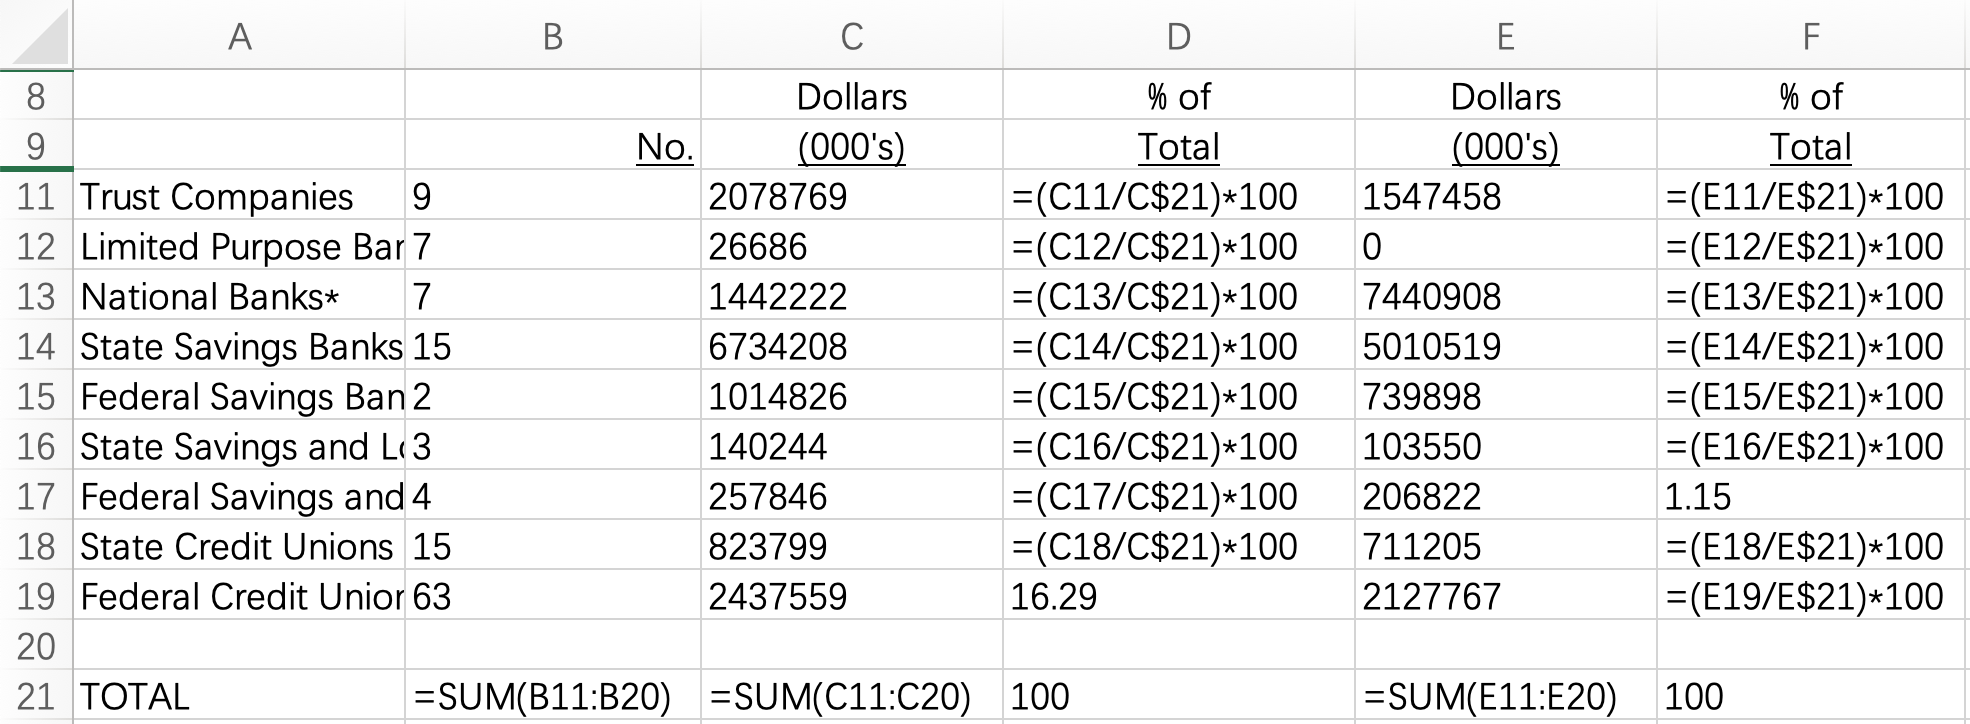
\includegraphics[width=\textwidth]{figure/style-A1.png}
    \caption{截取自EUSES 数据库中的电子表格 summ0602.xls 的工作表summary1201(A1 表示法)}
    \label{figure-A1}
\end{figure}

如图 \ref{figure-A1} 所示,该电子表格显示引用的方式是 A1 表示法。
在 A1 表示法中,一个在第 $X$ 列(A,B,\dots,Z,AA,\dots)第 $y$ 行(1,2,\dots)的单元格在行列都是相对引用的情况下表示为 $Xy$(如B5),在行列都是绝对引用的情况下中表示为 $\$X\$y$(如\$B\$5)。

\begin{figure}[tbp]    
    \centering
    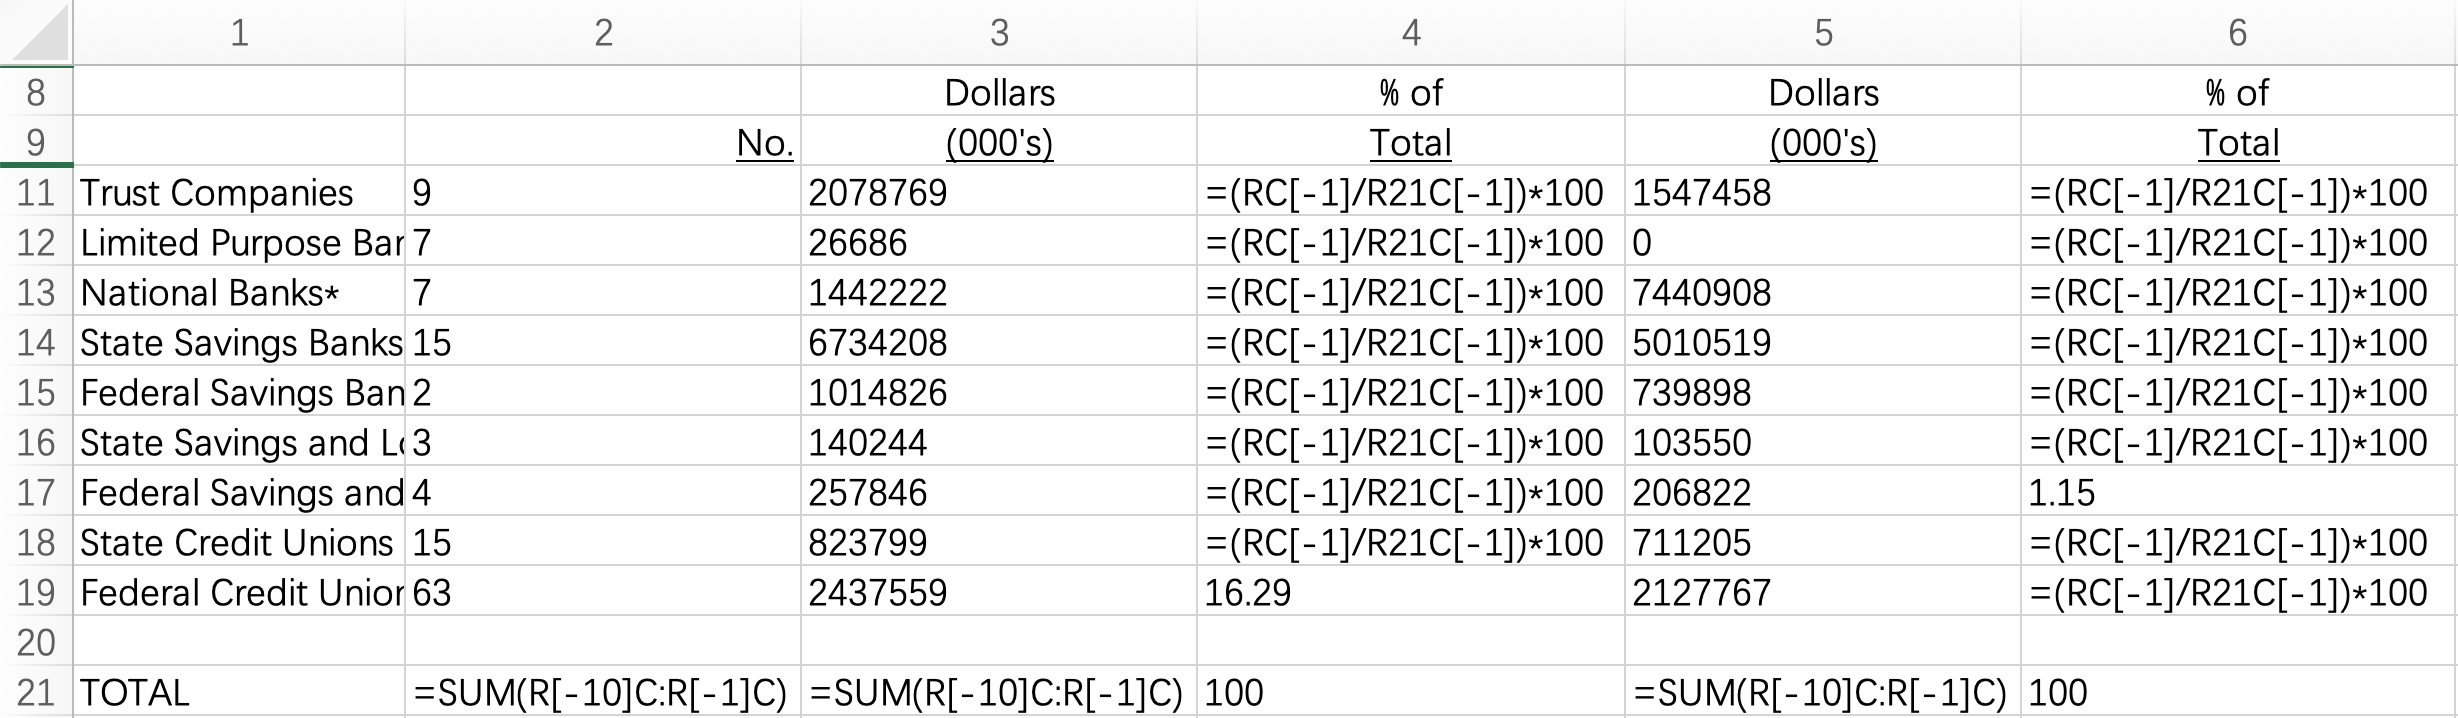
\includegraphics[width=\textwidth]{figure/style-R1C1.png}
    \caption{截取自EUSES 数据库中的电子表格 summ0602.xls 的工作表summary1201(R1C1 表示法)}
    \label{figure-R1C1}
\end{figure}

如图 \ref{figure-R1C1} 所示,该电子表格使用 R1C1 表示法,且所有单元格引用都是相对引用。
在 R1C1 表示法中,一个在当前单元格的下方第 $n$ 行(可以是负数,此时表示上方第 $n$ 行)和右侧第 $m$ 列(可以是负数,此时表示左侧第 $m$ 列)的单元格在行列都是相对引用的情况下中表示为 R[$n$]C[$m$](其中,$n$ 或 $m$ 在 $n=0$ 或 $m=0$ 时可以省略,而一个处在第 $n$ 行,第 $m$ 列的单元格在行列都是绝对引用的情况下表示为 R$n$C$m$。

如图 \ref{figure-A1} 和图 \ref{figure-R1C1} 所示,其中的单元格 D11 就是绝对引用和相对引用混合使用的例子,可以写成两种不同表示形式,即 =(C11$/$C\$21)$*$100 和 =(RC[-1]$/$R21C[-1])$*$100。

我们定义获取一个公式的所有引用的函数 $\sigma(exp)$ ,它返回一个集合,其中包含在该公式中使用到的所有引用。
该函数 $\sigma(exp)$ 可以形式化地表达为:
\begin{definition}
$
\sigma(exp) = 
\left\{
    \begin{aligned}
       & \emptyset & exp \in V; \\
       & \{exp\}     & exp \in R; \\
       & \sigma(exp_1) \cup \dots \cup \sigma(exp_n) & exp = \varphi(exp_1, \dots , exp_n).
    \end{aligned}
\right.
$
\end{definition}

一个有用的观察是:含有相似计算语义的公式单元格通常具有用 R1C1 方式表达的等价表达式。
例如,图 \ref{figure-A1} 中的单元格 D11 中的公式 =(C11$/$C\$21)$*$100 在 R1C1表示法中是图 \ref{figure-R1C1} 中的 =(RC[-1]$/$R21C[-1])$*$100。
图 \ref{figure-R1C1} 也给出了图 \ref{figure-A1} 中其他所有公式对应的 R1C1 表示结果。
我们不难观察出:在 A1 表示法下,从 D11 到 D18 的公式表达式不尽相同,但在 R1C1 表示法下,从 D11 到 D18 的公式表达式完全等价,因此在算法分析和设计时使用后一种表示法更为有利。
我们利用这一观察,从公式表达式中抽取特征来将单元格进行区分,将形式类似的公式吸纳进同一个类中,进而检测出该类中存在的缺陷单元格。


\section{电子表格的缺陷分类}
1997 年,Fowler等人\cite{fowler1997refactoring}提出代码缺陷(Code Smell)的概念。
代码缺陷指导致现有软件中存在潜在的维护问题的不良编码方式。
通常代码缺陷不会立即导致程序错误,但可能显著影响软件的可理解性和可维护性,例如在面向对象程序中,一个冗长的类定义可能难以理解和维护。
从电子表格缺陷的相关研究工作来看,后续的电子表格缺陷定义和分类都明显受到了代码缺陷概念的影响,下面详细介绍。

\subsection{所有类型单元格的缺陷粗分类}
2012 年,Cunha 等人\cite{cunha2012towards}受到代码缺陷的概念启发,率先较为全面地给出了电子表格缺陷的定义以及朴素的识别方法。
他们结合 EUSES 电子表格数据库中的实际案例,对电子表格中可能出现的单元格缺陷进行了分类整理和描述。
他们将电子表格的单元格缺陷分成如下四类:

\textbf{统计相关的缺陷}:
这类缺陷指的是在一列或一行纯数值中,那些不满足正态分布的数值单元格。
这类缺陷通常会引入用户疏忽导致的错误数值。
具体检测思路是计算某行或某列中所有数值的正态分布图,并将正态分布图的 95\% 以外的数值标记为有缺陷的单元格,并报告给用户。
在这类缺陷中,不考虑那些数值或者字符串单元格。
如图\ref{figure-valuesmell}所示,列 B 标准方差是 2.369E8。
那么,被正态分布接受的值应当在 [5.868E8, 1.534E9] 的范围内。
因为单元格 B4 保存着数值 123,这意味着它有可能是有缺陷的单元格。
同理,单元格 G12 也是存在缺陷的。

\textbf{类型相关的缺陷}:
在电子表格中含有四类基本类型的单元格:数值、公式、字符串和空单元格。
通过检查某个特定单元格周围的单元格类型趋势来判断当前单元格是否具有类型不一致性的缺陷。
比较朴素的方法是利用滑动窗口的方式,每次选择某行或某列的连续若干个单元格,检测出该窗口中具有明显与其他单元格具有不同类型的单元格,将其标记为有缺陷的。
如图\ref{figure-valuesmell}所示,我们可以观察到单元格 C6 和 G16 都是空单元格。
然而,它们出现的上下文环境中(这里假设检验时选定的滑动窗口大小为 5)所有的单元格都是被填充的,具有非空类型。
那么,我们即可将这两个单元格标记为有缺陷的。
同理,在单元格 F3 中含有字符串值“o”,但它周围的上下文环境表明列 F 绝大多数单元格都是数值类型,那么单元格 F3 就可以被标记为有缺陷的,其真实值很可能是数值 “0”。

\begin{figure}[tbp]    
    \centering
    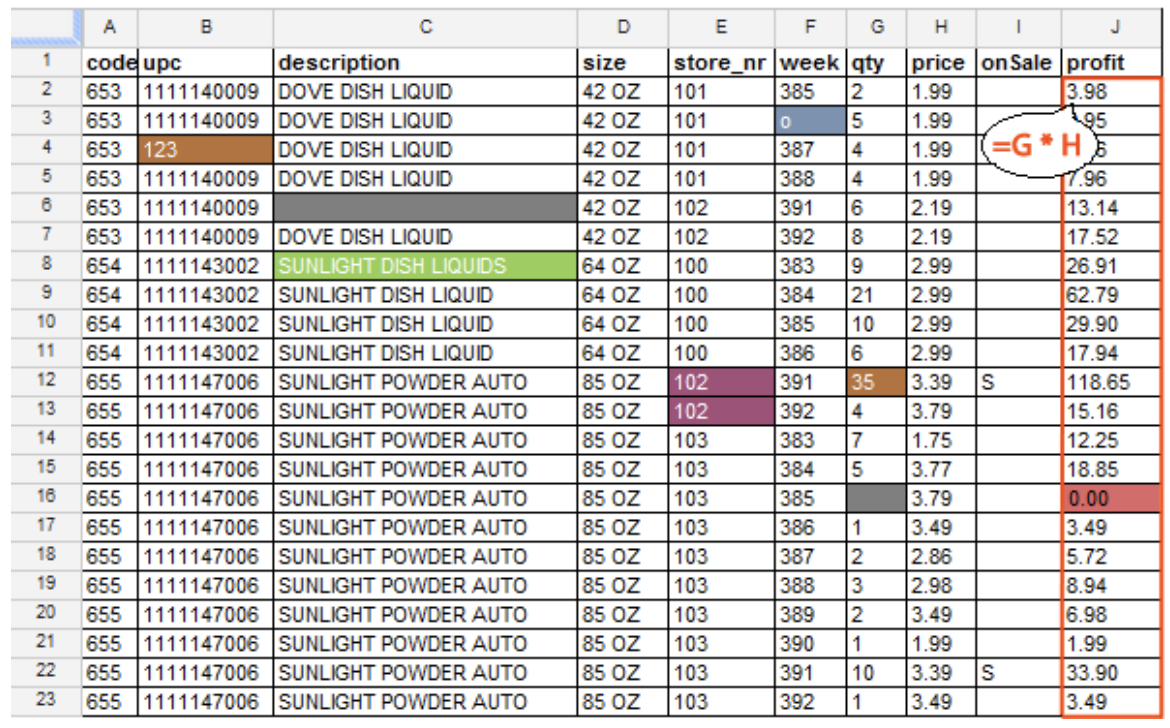
\includegraphics[width=\textwidth]{figure/relatedwork/valueSmell.png}
    \caption{电子表格中的缺陷示意图(其中有缺陷的单元格已用背景色标注出来)}
    \label{figure-valuesmell}
\end{figure}

\textbf{内容相关的缺陷}:
在此类别中,我们通过分析单元格的内容来检测缺陷。
在电子表格的使用环境中,终端用户很容易出现打字错误,比如对于字符串单元格来说,打错、多打、少打了一个字母,都很有可能发生。
我们通过计算两个字符串单元格内容之间的字符串距离,可以来判断是否某个字符串单元格是有缺陷的。
在检测缺陷时,我们可以使用 Levenshtein 算法来进行字符串编辑距离的计算。
如图\ref{figure-valuesmell}所示,单元格 C8 具有单元格 C9 到 C11 的内容的复数形式,而 C8 显然和这些邻近的单元格都有微小的字符串差异,因此我们可以推测该单元格是有缺陷的。

公式单元格也可能具有和内容相关的缺陷,比如该单元格公式引用了空单元格,通常就会导致计算结果无意义。
如图\ref{figure-valuesmell}所示,单元格 J16 被认定为是有缺陷的,因为它引用了空单元格 G16。

\textbf{功能依赖相关的缺陷}:
在此类别中,我们采用数据挖掘技术来检测电子表格中的“脏值”。
检测脏值的方法起初广泛地运用于数据库领域。
这里我们举例说明,如果列 A 中的相同值总是对应着列 B 中的相同值,那么我们说列 A 和列 B 是功能依赖的。
如图\ref{figure-valuesmell}所示,除去少量数据的不满足,列 B 就是功能依赖来列 A,特定的“code”值总是对应于它相应的“upc”值。
当我们检测到在确定已经存在功能依赖的两个列中存在不满足功能依赖的少量单元格时,这些单元格就应当被标记为有缺陷的。
比如单元格 E12 和 E13 被检测为有缺陷的。
因为我们可以发现 在列 A 到列 F元组(655,1111147006,SUNLIGHT POWDER AUTO,85 OZ) 大多数情况下总是对应于列 E 中的值 103,除了 E12 和 E13 不满足。

\subsection{公式类型单元格的缺陷细分类}
2012 年,同样受代码缺陷的启发,但与 Cunha 等人\cite{cunha2012towards}提出的针对所有单元格类型的单元格缺陷定义不同的是,Hermans 等人\cite{hermans2012detecting2,jansen2015code}提出了专门针对公式单元格缺陷的更细粒度的定义。

Hermans 等人结合 EUSES 电子表格数据库\cite{fisher2005euses}的实证经验,提出了五种与公式相关的缺陷种类:

\textbf{过多操作符的缺陷}:
受代码缺陷中“长方法”缺陷\cite{fowler1997refactoring}启发,此类的电子表格公式缺陷与公式的长度(或者说,操作符数量)有关。
它衡量一个公式中包含的操作总量。
图\ref{figure-multipleOperation}展示了一个 EUSES 数据库中具有此类缺陷的公式,它在一个公式内拥有 15 个不同的操作符,对于普通用户来讲很那理解,更加难以进行维护。

\begin{figure}[tbp]    
    \centering
    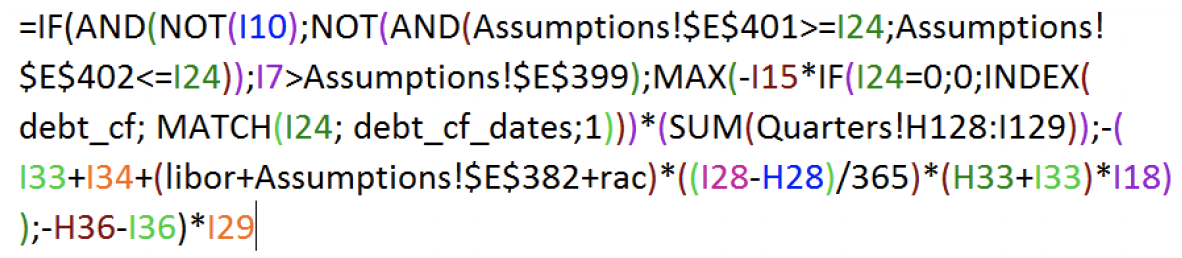
\includegraphics[width=0.8\textwidth]{figure/relatedwork/multipleOperation.png}
    \caption{过多操作符的公式缺陷示例}
    \label{figure-multipleOperation}
\end{figure}

\textbf{过多引用的缺陷}:
另一类臭名昭著的代码缺陷是方法定义拥有过多参数。
与此类似,在电子表格公式中就对应于过多单元格引用。
此类缺陷统计公式中引用的单元格数量。
图\ref{figure-multipleReference}展示了一个 EUSES 数据库中具有此类缺陷的公式,它总共含有 79 个单元格引用,显然给用户理解和维护带来困难。

\begin{figure}[tbp]    
    \centering
    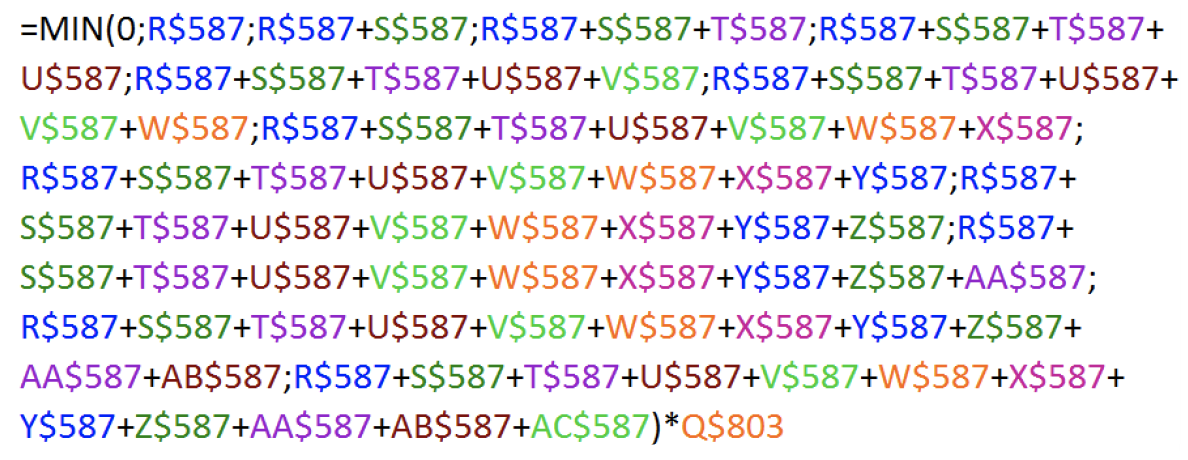
\includegraphics[width=0.8\textwidth]{figure/relatedwork/multipleReference.png}
    \caption{过多引用的公式缺陷示例}
    \label{figure-multipleReference}
\end{figure}

\textbf{过多条件嵌套的缺陷}:
过度嵌套的条件判断被认为是代码可读性的威胁\cite{fowler1997refactoring}。
对于电子表格公式来说,过多条件嵌套也影响了公式的可读性。
此类缺陷统计公式中条件嵌套的数量。
图\ref{figure-ConditionalComplexity}展示了 EUSES 数据库中的一个有 7 层嵌套的 IF 公式,Excel 2003 版本 最多只允许 7 层 IF 嵌套,这显然也有碍于电子表格的长期维护。

\begin{figure}[tbp]    
    \centering
    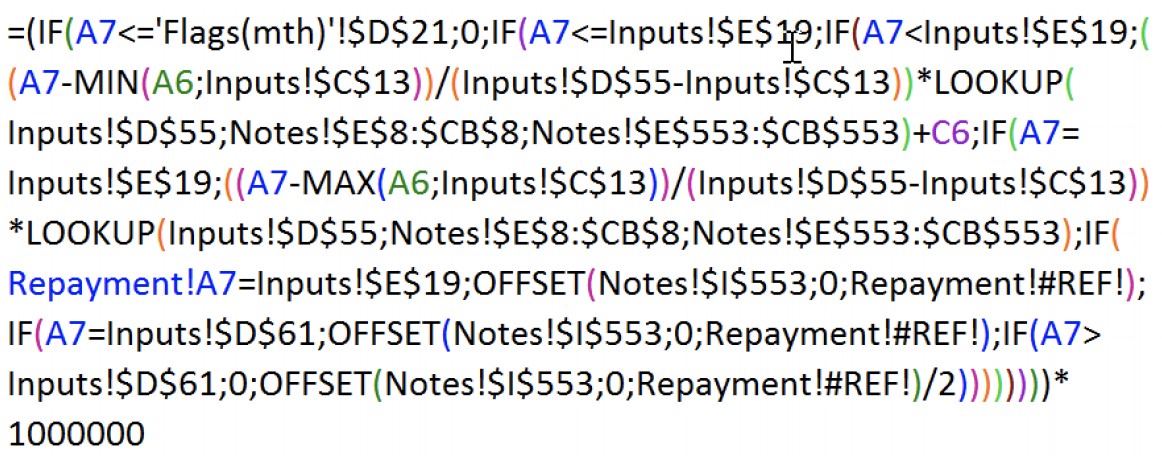
\includegraphics[width=0.8\textwidth]{figure/relatedwork/ConditionalComplexity.png}
    \caption{条件过度复杂的公式缺陷示例}
    \label{figure-ConditionalComplexity}
\end{figure}

\textbf{过长计算链的缺陷}:
电子表格中,公式引用很常见,因此这些引用关系就构成了电子表格的计算链。
追踪一个过长计算链对用户来说是一项枯燥且易错的任务。
此类缺陷通过衡量计算一个公式所需最长的引用路径长度。

\textbf{重复公式的缺陷}:
在代码维护中,我们通常想要同构的代码片段只有一份,方便日后的修改和维护。
同样地,电子表格中的公式也可能存在这样的问题。
如某个单元格中的公式是另一个公式的子公式,那这个单元格就被成为具有重复公式的缺陷。
通过对比R1C1表示法下的各个公式语法树,来判断是否存在此类缺陷。
如图\ref{figure-DuplicatedFormula}所示,第 39 行的四个公式具有完全相同的公式,因此这四个公式都具有重复公式的缺陷,
我们可以保留其中一个公式,另外三个直接引用被保留公式的计算结果即可,避免了维护的复杂性。

\begin{figure}[tbp]    
    \centering
    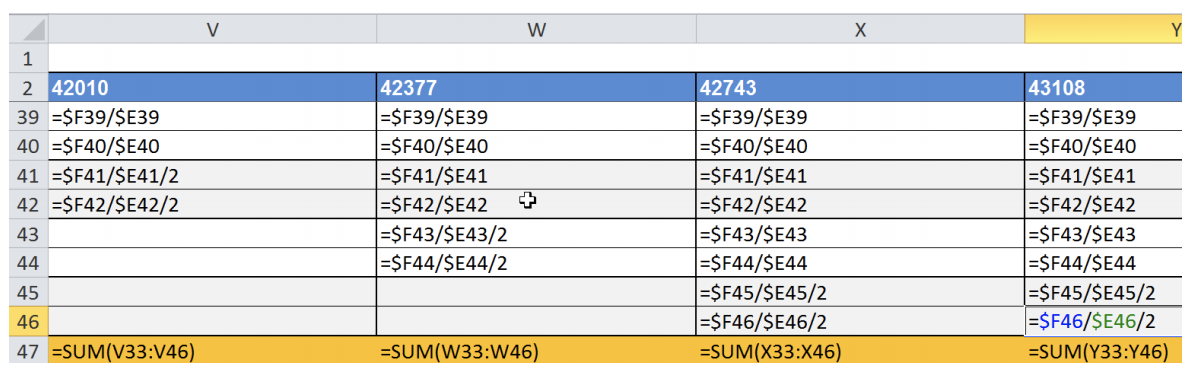
\includegraphics[width=\textwidth]{figure/relatedwork/DuplicatedFormula.png}
    \caption{重复公式的公式缺陷示例}
    \label{figure-DuplicatedFormula}
\end{figure}

\subsection{小结}
得益于 Cunha 和 Hermans 等人踏实的实证研究工作和缺陷分类整理\cite{cunha2012towards,hermans2012detecting2,jansen2015code},很多后续的缺陷预防和检测相关技术都是针对其中某些缺陷,提出行之有效的技术思路和实现方法。
在后续的相关工作中,研究者们也对缺陷定义做了各种细化和延伸的工作,但其基本骨架已经被这两种分类方式搭建起来,没有经历大的变化。


\section{电子表格缺陷的相关工作}
从电子表格的缺陷引入过程中,其本身就可以分成在缺陷引入前的技术研究(即缺陷预防)以及在缺陷引入后的技术研究(即缺陷检测和修复)两方面。
限于篇幅有限,本节分两小节分别讨论模型驱动相关的缺陷预防技术和各种类型的缺陷检测技术(本文的技术就属于后者),因为这两个技术方向在电子表格领域影响力较为深远,且相关工作众多。
电子表格的公式本身虽然可能很复杂,但其所属的缺陷类型对于终端用户来说,一经指出,就不难理解,因此终端用户通常也能进行相对快速的手工缺陷修复,因此本文不再专门讨论缺陷修复相关的技术研究,此部分可以参考其它文章\cite{badame2012refactoring,jannach2014avoiding,zhang2018automated}。

\subsection{电子表格的缺陷预防}
%------
1995年,Isakowitz 等人\cite{isakowitz1995toward}开始提出对电子表格中的数据及其结构进行建模。
他们把电子表格看做物理和逻辑的两个部分,物理部分就是单元格的公式和数值,逻辑部分就是描述电子表格功能的一系列函数关系。
借用他们设计的函数式关系型语言,通过提取算法能够从电子表格中将单元格之间的计算关系提取出来;类似地,也可以通过该关系型语言描述的电子表格模型生成实际的电子表格,即实现了从具体电子表格数据到模型之间的互相转换。
该工作为后续将面向对象技术和模型控制技术向电子表格的应用,奠定了基础。

1997年,Paine 等人\cite{ireson1997model,paine2008ensuring,paine2005bringing,paine2008rapid}也提出了针对电子表格的面向对象概念。
在他们的 Model Master 方法中,电子表格以声明式的方式表达为文本程序。
这些程序通过编译器处理,随即从规约中生成电子表格。
电子表格的数值和计算逻辑以类的形式表达,其中包括属性和相应的计算逻辑。
2008年,Paine等人\cite{paine2008spreadsheet}在之前Model Master工作的基础上,进而提出了针对电子表格的“结构发现”技术,使用编程语言Prolog来限定电子表格可能的逻辑结构。
该方法的目标是作为电子表格软件的“智能结构监控器”,允许用户在编辑表格的同时对表格结构进行重配置。
原作者们认为该技术可能是电子表格“最佳实践”的革命性成果。

\begin{figure}[tp]    
    \centering
    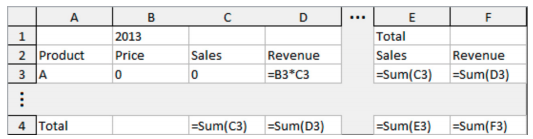
\includegraphics[width=1\textwidth]{figure/template.png}
    \caption{电子表格模板示例}
    \label{figure-template}
\end{figure}

2004年,Erwig等人\cite{erwig2004gencel,erwig2005automatic,abraham2005goal}同样注意到电子表格领域中实践和理论之间的巨大鸿沟,即电子表格软件缺乏可靠的质量保障技术,使得实际的表格中常会含有许多错误或缺陷。
因而,他们开发了一个模板规约语言,可以用来形式化地定义电子表格模板,同时可以表达可能的表格演化形式。
该语言基于表格计算子(table calculus),可以形式化地刻画创建和修改电子表格模板的过程。
Erwig等人为该底层模型设计了类型系统,以避免电子表格中频繁发生的类型相关的缺陷、公式引用相关的缺陷和缺失数据的缺陷。
在该底层模型的基础上,他们开发了Gencel可视化系统,用于依据描述语言自动生成可靠的电子表格。
图\ref{figure-template}即展现了使用Gencel系统描述出的可演化的电子表格模板,其基本框架和Excel类似。
终端用户通过点击“...”符号,可以对模板中可重复使用的组件进行添加。
在最初的工作中,需要人工手写模板规约,Abraham等人\cite{abraham2006inferring}为了能够自动地从电子表格中提取出对应模板规约,再反向应用到该表格的后续维护过程中,设计了一些行之有效的启发式方法。

%  2004年,Erwig等人\cite{erwig2004gencel,erwig2005automatic,abraham2005goal}提出基于表格模板的可视化方法来刻画电子表格底层模型的特定方面。
%  在他们的 Gencel 方法中,一个“表格模板”被用来特指电子表格中重复的区域。
%  模板的设计和修改过程类似于 MS Excel 软件的可视化操作方式。
%  图\ref{figure-template}展示了一个可视化模板的例子,其中列B、C和D下面的内容被标记为可重复的。
%  这类可重复的区域用所在列上和所在行上的两个省略号"..."和两条分隔带来表达。
%  2006年,Abraham等人\cite{abraham2006inferring}提出使用一些启发式方法能够从给定的电子表格中自动提取出存在的模板。

2010年,Engels等人\cite{engels2005classsheets,cunha2010automatically}结合基于模板的方法和面向对象的概念模型提出了 ClassSheet 的概念,
突破了基于模板方法只能刻画电子表格的“词法特征”的局限性,使用 ClassSheet 概念能够更完整地刻画整个表格的“语义特征”。
许多基于 ClassSheet 概念的改进方法被陆续提出\cite{luckey2012systematic,cunha2011type,cunha2011embedding,cunha2012bidirectional}。
2012年,Luckey等人\cite{luckey2012systematic}处理了模型演化和如何使得这类更新能够自动转换到已经生成的电子表格中的问题,以便更好地支撑电子表格完整的开发过程。

2019年,Dong等人\cite{dong2019semantic}关注于自动提取电子表格中的语义结构,他们设计了基于多任务的学习框架,来识别表格区域,结构组件及其单元格类型,进而利用最新的语言模型进展来刻画每个单元格的语义。
未来,越来越多基于机器学习的相关工作应该会陆续展现出来。

\subsection{电子表格的缺陷检测}
本世纪的前 10 年主要的缺陷检测相关工作,关注于使用类型推导的方法\cite{erwig2002adding,burnett2002testing,ahmad2003type,abraham2004header,abraham2006type,abraham2007ucheck,antoniu2004validating,chambers2009automatic,chambers2010reasoning}来检测电子表格缺陷。
这类方法的核心思路是借助人工标注或者字符串信息推导出数值单元格的类型信息,进而判断公式中的计算是否符合不同类型之间的运算法则,类似于传统程序在编译器中进行的静态类型检查。

Erwig等人\cite{erwig2002adding,abraham2004header,chambers2009automatic}最早把这种类型推导系统引入到电子表格的特定错误检测中来。
他们依据表头来推导类型信息,并结合用户标注的类型信息,推导出所有可能的数值单元格类型,进而验证公式运算的类型合法性。
但该方法需要较多的额外信息输入,才能分析出数值单元格的类型,对很多商用电子表格并不适用,因此适用范围较小,能够检测出的缺陷类型也相对较少。

本世纪的 20 年代至今,研究者们更加关注电子表格中与公式相关的缺陷。
这些电子表格公式缺陷本身未必是错误的,但在未来的软件开发、重构或拓展过程中可能导致错误。

正如本章第二节所述,Hermans 等人\cite{hermans2012detecting,hermans2012detecting2,hermans2013data}率先关注此类公式缺陷。
2012年,Hermans等人\cite{hermans2012detecting2}率先将代码缺陷概念移植到电子表格领域,针对公式类型单元格定义了五种相关缺陷。
该方法通过一系列的硬性统计指标来衡量一个公式单元格是否有缺陷,并将有缺陷的部分在电子表格中高亮出来,供用户进一步分析。
同年,Hermans等人\cite{hermans2012detecting}使用类似于\cite{hermans2012detecting2}的思路考察跨工作表之间(inter-worksheet),但表格结构相似的对应单元格中是否有缺陷。
次年,Hermans等人\cite{hermans2013data}基于现有的文本克隆检测算法,适配到电子表格中,检测公式之间的复制-粘贴关系,识别出那些在复制公式时仅复制值的电子表格缺陷(因为仅复制公式的值会导致后续可读性和维护性显著恶化)。

2014年,窦文生等人\cite{dou2014spreadsheet}注意到具有相同计算语义的电子表格单元格在布局上常常是连续的多个单元格,并且同属于相同的行或列\footnote{类似于用一个矩形圈出的单列或单行连续多个单元格区域,称为\textit{单元格阵列}(\textit{cell array})}。
在表格演化的过程中,由于特定的修改或者破坏性的复制-粘贴操作,单元格这列中的单元格不再具有相同的计算语义,那么该单元格阵列中就含有有缺陷的单元格了。
该技术AmCheck使用启发式的方法,结合公式引用的同构特性,来识别这些单元格阵列区域,进而使用启发式策略和程序合成技术来检测并修复每个单元格阵列中的单元格缺陷。
2016年,窦文生等人\cite{dou2016detecting}将关注的目光放到克隆的表格上\footnote{这里的表格(table)指一个多行多列的矩形区域,包含字符串表头,以及多个核心的数值和公式单元格,如果把工作表比作一个Java类,那么表格就是其中一个方法,用以实现某个特定功能}。
在克隆的表格之间的对应单元格理应保持相同或相似的计算语义。然而,和\cite{dou2014spreadsheet}中指出的相似原因,克隆的表中会存在有缺陷的单元格。
该技术TableCheck根据表头信息和已有的基于指纹概念的代码克隆检测技术来判断两个表格是否是克隆关系,一经确定,进而使用启发式策略来判断每个单元格是否保持了相同的语义,其中的异常者就是有缺陷的单元格,终端用户可以参考克隆表格的信息来修改检测出的缺陷。
2017年,窦文生等人\cite{dou2017cacheck}在 \am 技术的基础上进行实证研究,发现除了同构类型的单元格阵列之外,另一类具有异构特性的单元格这列在EUSES数据集中也频繁出现,因此他们提出CACheck技术能够同时识别出同构和异构的单元格阵列,并利用和 \am 相似的技术进行后续的缺陷检测和修复推荐。
2018年,Xu等人\cite{xu2018spreadsheet}对电子表格模板在真实商业数据集Enron上的使用进行实证研究。
他们发现终端用户由于缺陷必要的工具支撑,难以找到预先定义好的表格模板,通常选择从已有表格中进行表格克隆,然后进行修改,这样不可避免地导致发生在一个表格中的缺陷不断衍生下去。
2020年,Zhang等人\cite{zhang2020learning}在TableCheck技术的基础上进行实证研究,发现超过一半的发生克隆的表格中发生了结构变化,比如新增了几行或者几列数据,然而TableCheck技术只能检测结构相同的克隆表格。
该技术LTC通过提取通常保持相似的结构和格式,比如表头,公式和背景颜色等信息,来构造二分类器,进而识别出带有结构变化的克隆表格。
实验表明,LTC技术相比TableCheck取得了精度和召回率上的极大提升。
使用类似的技术思路,也可以检测电子表格中的空单元格缺陷\cite{xu2018detecting}。
本文在实验评估部分,选用了\am 和 \ca 这两个缺陷检测技术作为我们\wa 技术的对比技术,因为这两个技术在使用模式匹配和设计精妙的启发式方法来辅助识别单元格阵列和公式缺陷方面效果显著,是主流的缺陷检测技术之二。

2016年,Cheung等人\cite{cheung2016custodes}注意到\am 和 \ca 技术只能检测单元格这列这种结构的单元格类,如果具有相似计算语义的单元格不是连续分布,就无法被这两种技术识别出来。
因此,他们提出了 \cu 技术,基于机器学习的两阶段聚类方法来对单元格进行聚类,识别出足够多的单元格类,进而通过离群点检测技术在每个单元格类中识别出离群点,即具有缺陷的单元格。
该方法因为采用特征抽取的方式来进行聚类,克服了单元格类必须连续的局限性,同时也提升了识别单元格类的召回率。
值得一提的是,直到2016年,针对电子表格的公式缺陷设计的基准测试集(采样自EUSES数据库)才得到后续研究工作的广泛使用,有利于后续工作\cite{singh2017melford,Barowy2018excelint}在实验评估中进行有效的技术对比。
本文即是对 \cu 技术的进一步优化,后面的方法设计和实验评估章节都会进一步介绍,此处不再赘述。

\begin{figure}[tbp]    
    \centering
    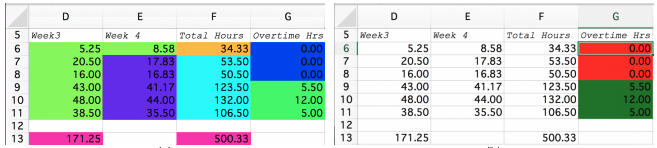
\includegraphics[width=1\textwidth]{figure/figure-excelint.png}
    \caption{ExceLint 工具对公式单元格的划分结果展示}
    \label{figure1}
\end{figure}

2017年,Singh等人\cite{singh2017melford}利用近些年在语音和图像识别领域大火的深度学习技术来检测本该是公式但用纯数值表示的单元格缺陷。
该技术Melford通过对被检测的单元格周围进行单元格的空间抽象来构建分类器,用于判断该单元格是否应该包含一个公式。
该方法理论上能够和 \cu 技术形成互补,不过目前的实验表明该方法能够检测出的缺陷数量仅是\cu 的子集,但原作者认为即便使用了简单的深度学习训练模型,已经取得了不俗的效果,表明该技术方向有广阔的应用前景。

2018年,Barowy等人\cite{Barowy2018excelint}采用信息论的方法来检测公式相关的缺陷。
该方法充分利用电子表格的矩形特征,根据信息熵的计算结果来识别最能显著破坏矩形区域的公式,利用这些有突出代表性的公式来对整个表格进行矩形切分,如图\ref{figure-excelint}所示。
最终,在每个识别出的矩形区域,每个公式单元格应当具备相似的计算语义,进而根据单元格引用特征来识别出离群点,即那些有公式引用缺陷的单元格。
此技术ExceLint在实验中\cite{Barowy2018excelint}与\cu 技术进行对比,在检测公式引用缺陷方面比\cu 取得了更好的效果。

2019年,Koch等人\cite{koch2019refinement}发现当前已有的电子表格缺陷检测技术具有几个共同的缺陷,导致不正确的或冗余的缺陷报告。
例如,相同的质量问题经常在每个单元格的克隆副本上都被汇报出来,这巨大的缺陷数量可能使得终端用户难以承受。
因此,Koch等人提出对检测出的电子表格缺陷进行进一步筛选再汇报给终端用户,通过使用在缺陷检测阶段推导出的结构化信息。
该方法在实验中也证实了能够显著减少不正确的和冗余的缺陷报告。

% \subsection{小结}
%这里还是要再引用10篇左右近三年的论文,不能胡扯
% 除了直接针对电子表格的缺陷检测技术,近些年研究者们也在考虑如何自动化地从不同的角度帮助终端用户来提升电子表格的可靠性和可维护性。

% 比如,Zhang等人\cite{zhang2018automated}就重点关注我们在第2.2.2节提到的多层嵌套IF公式的自动化重构技术。
% 另外,Xu等人\cite{xu2018detecting}关注于如何检测有缺陷的空单元格,接近于我们在第2.2.1节提到的本该有公式却只是一个空单元格的类型相关的缺陷。


% 电子表格的相关工作主要集中在两个研究领域,信息系统和计算机科学领域。
% 在本章中,我们从计算机科学领域(主要是软件工程)的视角出发,对电子表格的质量保障技术进行分类讨论。
% 根据它们的设计目的,我们把各种电子表格的质量保障技术分成两类:
% \begin{itemize}
    % \item \textit{避免错误}的技术帮助终端用户从开发的起始阶段就能创建出不含错误的电子表格,对应本章第一节讨论的相关工作;
    % \item \textit{发现和修复错误}的技术帮助终端用户检测电子表格中蕴含的错误并理解错误发生的原因,进而修复这些的错误。
    % 这类技术通常在电子表格已经开发、编辑完成之后使用,对应本章第二节和第三节讨论的相关工作。
% \end{itemize}

% 接下来,我们将相关工作分成三个小节来讨论,即模型驱动的电子表格开发技术、电子表格的缺陷定位、检测和修复技术、以及电子表格的辅助支撑技术。

%  \section{模型驱动的电子表格开发技术}
%  基于模型驱动的方法并不是设计用来帮助终端用户发现潜在的错误,而是把提升电子表格的质量、结构的清晰度和防止错误注入放在首位。
%  类似于一般软件工程领域的模型驱动方法,这类技术的核心想法是在电子表格的开发过程中引入额外的抽象层。
%  这个额外的抽象层引入了更多抽象概念,在开发者的内在意图和电子表格的真实实现中间充当了沟通的桥梁。
%  在商业化的电子表格系统中日益扩大的这层语义鸿沟\cite{luckey2012systematic}得到了有效缓解。

%  这类抽象的电子表格模型通常出现在开发过程的两个阶段:
%  \begin{itemize}
    %  \item 它们被用作“代码生成器”的形式化描述。在这个场景下,电子表格的一部分从模型中自动生成,因此减少了纯人工操作产生错误的风险;
    %  \item 它们也被用于从已有的电子表格中恢复出内在蕴含的概念结构,帮助终端用户理解当前电子表格的计算模型,进而减少后续可能产生的误解。
%  \end{itemize}

%  \subsection{电子表格的面向对象模型}
%  Isakowitz 等人\cite{isakowitz1995toward}是最早提出从建模角度来处理电子表格程序。
%  他们的核心假设是电子表格程序可以看做物理和逻辑的两个部分,物理部分就是单元格的公式和数值,逻辑部分就是描述电子表格功能的一系列函数关系。
%  而逻辑这部分可以从给定的电子表格中自动提取出来,并用领域特定语言(Domain-specific Language,DSL)表达出来。
%  该系统也能够从这样的逻辑规约中合成电子表格。

%  Paine 等人\cite{ireson1997model,paine2008ensuring}也提出了类似的针对电子表格程序的面向对象概念。
%  在他们的 Model Master 方法中,电子表格以声明式的方式表达为文本程序。
%  这些程序通过编译器处理,随即从规约中生成电子表格。
%  电子表格的逻辑以类的形式表达,其中包括属性和计算逻辑。
%  该建模语言中也提供许多特征(如类继承,多维数组扩展)来支持表格化的计算。
%  我们也可以逆向使用该方法,从给定的电子表格中提取出对应的逻辑模型,进而用于发现电子表格中的特定计算结构\cite{paine2008spreadsheet}。

%  Paine 等人\cite{paine2005bringing,paine2008rapid}后续提出了另一种声明式建模语言。
%  他们开发的 Excelsior 是一个电子表格开发系统,构建在 Prolog 上的编程语言,同时针对 Excel 设计了模块化和可重用的规约表达方式。

%  \begin{figure}[tp]    
    \centering
    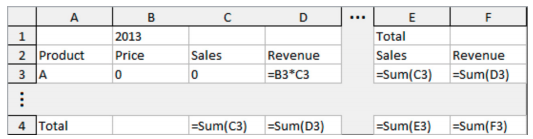
\includegraphics[width=1\textwidth]{figure/template.png}
    \caption{电子表格模板示例}
    \label{figure-template}
\end{figure}
%  \subsection{电子表格的可视化模板}
%  Erwig 等人\cite{erwig2004gencel,erwig2005automatic,abraham2005goal}提出基于表格模板的可视化方法来刻画电子表格底层模型的特定方面。
%  在他们的 Gencel 方法中,一个“表格模板”被用来特指电子表格中重复的区域。
%  图\ref{figure-template}展示了一个可视化模板的例子。
%  模板的设计和修改过程类似于 MS Excel 软件的可视化操作方式。
%  在图\ref{figure-template}中,$B$、$C$和$D$列下面的内容被标记为可重复的。
%  这类可重复的区域用所在列上和所在行上的两个省略号"..."和两条分隔带来表达。

%  类似于 Paine 等人的工作,电子表格也可以从模型中自动生成。
%  另外,基于模板的方法也支持逆向工程,Abraham 等人\cite{abraham2006inferring}提出使用一些启发式方法能够从给定的电子表格中自动提取出存在的模板。

%  后来,Engels 等人\cite{engels2005classsheets,cunha2010automatically}结合基于模板的方法和面向对象的概念模型提出了 ClassSheet 的概念,
%  突破了基于模板方法只能刻画电子表格的“词法特征”的局限性,使用 ClassSheet 概念能够更完整地刻画整个表格的“语义特征”。
%  许多基于 ClassSheet 概念的改进方法被陆续提出\cite{luckey2012systematic,cunha2011type,cunha2011embedding,cunha2012bidirectional}。
%  比如 Luckey 等人\cite{luckey2012systematic}处理了模型演化和如何使得这类更新能够自动转换到已经生成的电子表格中的问题,以便更好地支撑电子表格完整的开发过程。

%  Hermans等人\cite{hermans2010automatically}提出了另一个不同的可视化方法来重构底层面向对象模型。
%  该方法基于人工设计的经典模式库,通过二维解析和模式匹配算法来尝试定位电子表格中的各类构建模式。
%  最终的构建模式被转换成 UML 类图,可用于更好地理解和提升当前的电子表格质量。

%  \subsection{电子表格的关系型模型}
%  电子表格的主要原则之一:数据以表格的形式组织。
%  一个直接的获得表格的结构模型的方法是借鉴关系型数据库的设计原理和实践方法。
%  以构建高质量和零错误的表格为目的,Cunha 等人\cite{cunha2009spreadsheets}提出了从电子表格中提取关系型数据库范式的方法。
%  该方法的主要优点是能够获得更加模块化、没有数据冗余、并预防错误的数据输入的电子表格模型\cite{cunha2009discovery,cunha2012relational}。


%  \section{电子表格的缺陷分析技术}
%  电子表格的编程范式使得终端用户容易犯错。
%  随着电子表格包含的数据量越来越大,依赖终端用户人工检查每个公式的计算结果是否符合预期,效率低下。
%  相应地,针对电子表格的自动化错误/缺陷定位、检测和修复工作得到了研究者们的广泛关注。
%  这些方法也可以基于是否需要人工辅助分成两类,人工辅助具体包括用户给定测试输入、按要求提供额外的标注信息等。

%  \subsection{缺陷定位}
%  早期的电子表格错误定位工作\cite{reichwein1999slicing,ruthruff2005interactive},使用计算轨迹的候选者排序策略来寻找有缺陷的单元格,类似于传统程序分析中的基于频谱的错误定位方法。
%  他们首先提出将程序切片的概念应用到电子表格中,以消除不可能的错误候选者。
%  该类技术使用用户给定的辅助信息关于正确和不正确的单元格值,并把对一个错误的单元格值有贡献的单元格标记为可能错误的。
%  一个单元格的公式如果对更多的已经标记为错误的值有贡献,那么很可能就是错误的。
%  相反,对更多正确的单元格值有贡献,那么很可能就是正确的。
%  如果一个单元格对错误的单元格值有贡献,但是它本身只由正确的单元格值计算而来,那么它的错误可能性就会减小。
%  该类方法,就是依据这种想法,进行量化排序。
%  后续,Hofer 等人\cite{hofer2013empirical}使用更加形式化的方法,以相似性系数来计算电子表格单元格的错误可能性。

%  另一条错误定位的思路是把电子表格转换成基于约束的形式,使得关于异常值的原因定位的复杂推导变得可能。
%  Jannach 等人\cite{jannach2010toward}提出将电子表格错误定位问题转换成约束可满足性问题(CSP)\cite{tsang2014foundations}。
%  基于用户给出的测试用例和关于某些单元格的异常值信息,该方法使用基于模型诊断的原则来判定哪些单元格原则上可能是异常计算结果的真正原因。
%  后来,Jannach 等人\cite{jannach2016model}又提出了新的算法改进策略,帮助提升原方法的可扩展性。

%  类似的方法也得到了 Abreu 等人\cite{abreu2012constraint,abreu2012debugging}的采用。
%  Abreu 的方法尽管整体上与 Jannach 等人的方法相似,但技术实现上有差异。
%  他们没有使用 Hitting-Set 算法\cite{reiter1987theory},而是把单个公式的正确性的推导直接编码成约束表达。
%  因此他们利用了额外的布尔变量来代表每个公式的正确性。
%  另外他们的方法可以同时运用于多组测试用例的并发执行。

%  Hofer 等人\cite{hofer2013empirical}提出把一个轻量级的基于模型的调试技术,结合到他们的基于频谱的错误定位方法中。
%  他们建议使用从统计错误定位技术(SFL)得到的系数作为基于模型的调试过程的初始可能性值。

%  \subsection{缺陷检测}
%  本世纪的前 10 年主要的缺陷检测相关工作,关注于单位和类型推导的方法\cite{erwig2002adding,burnett2002testing,ahmad2003type,abraham2004header,abraham2006type,abraham2007ucheck,antoniu2004validating,chambers2009automatic,chambers2010reasoning}来检测电子表格错误或缺陷。
%  这类方法的核心想法是推导出输入单元格的单位信息,进而判断公式中的计算是否符合单位之间的运算法则,类似于普通程序在编译器中进行的静态类型检查。
%  Erwig等人\cite{erwig2002adding,abraham2004header}最早把这种单位推导系统引入到电子表格的特定错误检测中来。
%  他们根据表头推导策略和用户标注,推导出所有可能的输入单元格单位信息,进而验证公式的单位运算合法性。

%  本世纪的 20 年代至今,学界更加关注一类称为电子表格缺陷(Spreadsheet Smell/Defect)的公式错误,该概念派生于软件维护领域的代码潜在错误\cite{fowler1997refactoring},用于特指不良代码设计风格和使用习惯。
%  这些代码本身未必是错误的,但在未来的软件开发、重构或拓展过程中可能导致错误。
%  Hermans 等人\cite{hermans2012detecting,hermans2012detecting2,hermans2013data}最早明确地将此类概念发展到电子表格领域中。
%  通常,电子表格缺陷是通过一些启发式的方法来描述不良设计风格。
%  Hermans 等人\cite{hermans2012detecting} 提出所谓的“工作表之间的单元格缺陷”。
%  这类缺陷根据不同工作表之间的依赖关系分析,来识别一些不良使用导致的单元格缺陷。
%  比如,一个公式引用了很多另一个工作表中的单元格,那么该公式应当被移动到对应工作表中。
%  公式缺陷最早在\cite{hermans2012detecting2}的工作中得到较为深入的分类和讨论。
%  后续,Hermans 等人\cite{hermans2013data}提出一个定位电子表格中数据克隆的方法。

%  窦文生等人\cite{dou2014spreadsheet,dou2017cacheck}提出“单元格阵列”的缺陷检测方法,通过定位同行或同列的具有类似公式语义的连续单元格阵列,进而利用基于组件的程序合成方法在每个单元格阵列中来检测公式异常。
%  后来,窦文生等人\cite{dou2016detecting}又提出进行跨表格(table)的克隆检测和单元格缺陷检测,通过识别结构同构的表格,进而对相应位置的单元格进行对比,来寻找公式异常。

%  \begin{figure}[tbp]    
    \centering
    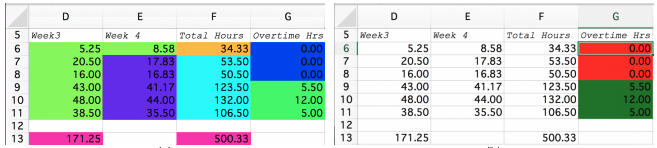
\includegraphics[width=1\textwidth]{figure/figure-excelint.png}
    \caption{ExceLint 工具对公式单元格的划分结果展示}
    \label{figure1}
\end{figure}
%  考虑到前人工作的召回率偏低问题,Cheung等人\cite{cheung2016custodes}提出基于学习和聚类的技术来对单元格进行分类,尽可能保证每个类中的单元格都含有相似的计算语义,进而在类中检测公式缺陷。
%  本文即是对 Cheung 等人工作的进一步优化和提升,后面的章节会进一步介绍。
%  类似地,如图\ref{figure-excelint}所示,ExceLint\cite{Barowy2018excelint}技术通过对公式中蕴含的信息熵分析来给出最合理的电子表格切分方式,最后在每个切分出的单元格矩阵中来进一步检测是否存在公式缺陷。
%  Melford\cite{singh2017melford}技术通过提取每个单元格附近的其他单元格属性,利用神经网络模型来寻找异常单元格,它的检测范围是\cu \cite{cheung2016custodes}的真子集。

%  \subsection{缺陷修复}
%  基于修复的方法不仅向用户指出有潜在问题的公式,也额外给出修复方案,比如应该把错误的公式修改成何种具体的正确公式。
%  Abraham 等人\cite{abraham2005goal}做出了第一份自动化给出修改建议的工作 GoalDebug(以目标为导向的调试技术)。
%  该方法中,需要用户为错误的单元格给出预期的结果,通过递归修改单个公式,根据电子表格特定的修改推导规则反向传播到之前的公式中,进而尝试自动给出合适的修改建议。
%  能够获取预期结果的修改结果再根据启发式方法进行排序。
%  另一个改进上述提到的 GoalDebug 的方法 \cite{abraham2007goaldebug,abraham2008mutation} 更适合处理多种的电子表格错误类型。
%  在缺陷检测中提到的工作\ca \cite{dou2014spreadsheet,dou2017cacheck},通过基于组件的程序合成技术\cite{jha2010oracle}也能够为检测到的单元格缺陷提供基础的修复公式建议。


%  \section{电子表格的辅助支撑技术}
%  这类辅助支撑技术在电子表格的开发和维护过程中给予用户帮助,包括帮助用户避免发生引用错误、
%  对电子表格的长期使用提供支撑(监控表格变动的工具、自动化重构的插件等),以及自动帮助用户完成数据提取任务的程序合成工具。

%  \subsection{演化}
%  电子表格通常经历各种变化,不巧的是,变化常常会引入错误。
%  FormulaDataSleuth\cite{bekenn2008reducing}是一个旨在帮助电子表格开发者在表格变动时,立刻检测到这类错误的工具。
%  一旦开发者已经声明了哪些数据单元格和区域应当被工具监控,系统就会自动监测许多类型的潜在问题。
%  对于已经定义好的数据区域,工具能够检测出空单元格、或者输入值拥有错误的数据类型、或者超出了预定义的数据范围。
%  对于被监控的公式单元格,偶然的公式重写以及引用了错误的单元格也会被识别出来。

%  理解给定的电子表格如何随着时间演化,并观察不同版本之间的差异,对于在不同项目中重用电子表格至关重要。
%  Chambers 等人\cite{chambers2010sheetdiff}提出了 SheetDiff 算法,能够检测并可视化特定类型的不同版本的电子表格之间的显著差异。
%  后来,为了克服上述贪心算法 SheetDiff 中存在的问题,Harutyunyan 等人\cite{harutyunyan2012planted}提出一种基于动态规划的算法 RowColAlign,能够更加高效和准确地检测版本差异。
%  徐良等人\cite{xu2017spreadcluster}利用聚类技术对电子表格整体进行聚类,进而寻找出多个电子表格文件之间的演化关系,并给出了我们在第六章案例研究中使用的测试对象,一个电子表格数据集 VEnron2。

%  \subsection{重构}
%  重构被定义为修改程序内部结构,但不修改功能性的过程\cite{o2010spreadsheet}。
%  除了应用于传统代码,重构在多个方面也有助于电子表格的质量保障。
%  比如,通过简化公式,使得整体更易理解;通过移除冗余公式,使得维护更加轻松,更少犯错。
%  电子表格领域的重构通常和行列调整有关,也就是电子表格的设计和布局的转换。
%  让终端用户人工进行这类转换,常常是耗时且易错的。

%  Badame等人\cite{badame2012refactoring}根据使用经验提出电子表格中的七种重构策略,并给 MS Excel 软件提供了一个相应的重构插件 RefBook。
%  该插件自动检测需要重构的单元格位置,并给终端用户提供重构建议。
%  例如可能提供的重构建议有:将单元格常量化、添加“守护”单元格、以及替换不合理的公式等。

%  Harris等人\cite{harris2011spreadsheet}提出了一种根据用户给定的样例进行复杂表格转换的方法。
%  该方法基于一个描述表格转换的领域特定语言 TableProg,以及一个 ProgFromEx 算法。
%  该算法需要用户提供几组转换示例,描述单元格变化前后的具体字符串。
%  ProgFromEx 能够自动推导出若干个转换程序,选择其中排序最高的一个,来帮助终端用户完成这样的表格转换过程。
%  与此类似的相关工作很多,研究者们将程序合成、程序语言领域的理论成果应用到电子表格的实际使用中,如 FlashFill\cite{singh2016transforming}。

%  \subsection{复用}
%  通常,复用已有的已经验证过的软件制品能够节约开发时间,避免犯错的风险,提升整体项目的可维护性\cite{ye2005reuse}。
%  这种复用思路也可以应用于电子表格领域。
%  独立的电子表格或者其中的部分通常可以在其他项目中重用。
%  对于公式复用的标准做法是简单的复制粘贴该公式。
%  然而,改变最初的公式并不会改变它的副本,如果忘记对公式副本进行更新很容易导致错误。

%  电子表格程序中的复用问题得到了 Djang 等人\cite{djang1998similarity}和 Montigel等人\cite{montigel2002portability}的关注。
%  Djang 等人\cite{djang1998similarity}沿用了面向对象思想中对继承概念的使用,来实现电子表格中的复用功能。
%  原则上,它允许用户在单个单元格和更粗粒度的层面上,以多个继承或相互继承的形式,声明电子表格单元格之间的依赖关系。
%  而 Montigel 等人\cite{montigel2002portability}提出了电子表格语言 Wizcell。
%  Wizcell 语言通过实现粘贴/复制、拖/拽等功能,使得和复用相关的语义变化更加明显,来缓解复用问题。
%  %  特别地,提出了四种这类操作的可能输出:
%  %  要么被复制的公式再被复制一次;
%  %  要么被复制的公式存在对原公式的引用;
%  %  要么复制后的单元格中的公式引用了之前原始单元格集合中的某部分单元格;
%  %  要么其引用随着副本和原来单元格之间的相对距离而对应改变。
%  Wizcell 语言允许用户声明潜在语义,因此大大降低了由于复用引入错误的可能。


%  %  \section{电子表格的测试方法}
%  %  在专业的软件开发流程中,系统测试对于保障软件制品的高质量至关重要。
%  %  通常这类测试活动既有开发者,也有专门的测试者介入。
%  %  但因为非专业的电子表格用户通常没有软件工程的思维和实践经验,对应的测试过程通常是不系统且散乱的。

%  %  考虑到电子表格即时反馈的特质,测试过程通常仅通过输入一组测试用例,然后检查对应的中间单元格和最终的汇总单元格是否产生了预期输出。
%  %  同时,商业电子表格工具,如 MS Excel,并不提供任何特定的机制帮助用户存储这些测试用例或进行回归测试。
%  %  而且,这类工具通常也不会帮助用户评估是否已经进行了足够的测试。
%  %  下面,我们回顾一下那些旨在将标准软件测试的概念,想法和工具移植到电子表格开发过程的相关工作。

%  %  \subsection{测试完备性和测试用例管理}
%  %  1997 年,Rothermel 等人\cite{rothermel1997testing,rothermel1998you,rothermel2001methodology}提出了针对电子表格的测试方法,被称为“所见即所测”(What You See Is What You Test,简记为 WYSIWYT)。
%  %  在电子表格构建期间,用户交互性地对当前给定输入下的一些派生出的单元格的值标记为“正确的”。
%  %  基于这些测试,系统自动判定该电子表格的被测试程度。
%  %  这个判定过程依赖于一个测试完备性准则,该准则基于电子表格的抽象模型,一种特定的“定义-使用”关系和动态执行轨迹。
%  %  后来,相继提出了一些优化方法,例如扩展到更大的同质性电子表格,增加对递归的支持,或是处理测试用例重用的问题\cite{burnett1999scaling,burnett2001visually,burnett2002testing,fisher2002automated,fisher2006scaling,randolph2002generalised}。

%  %  \subsection{自动化测试用例生成}
%  %  在使用 WYSIWYT 时,电子表格用户会受到关于表格被测试程度的反馈,但用户人必须要手动给出测试用例。
%  %  为了在这个用例生成过程中给予用户帮助,Fisher 等人\cite{fisher2002automated,fisher2006integrating}提出了测试用例自动化生成技术。
%  %  主要通过两种方法来生成新的测试用例。
%  %  一种是随机方法,随机地生成值并检查是否整个执行使用到了目前没有被测试过的“定义-使用”对的路径,有点像传统软工中的测试路径覆盖。
%  %  另一种是目标导向的方法,以尚未测试过的“定义-使用”对为目标,尝试修改输入值来覆盖它,该过程可以迭代进行。

%  %  在 Abraham 等人的工作\cite{abraham2006autotest}中,AutoTest 工具实现了自动化测试用例生成的不同策略,采用约束求解的方式来搜索导致预期的“定义-使用”对能够执行的单元格值。该方法能够为所有可行的“定义-使用”对生成测试用例,相比于 Fisher 等人的方法\cite{fisher2006integrating},AutoTest 工具更加有效且高效。

%  %  \subsection{基于断言的测试}
%  %  另一类对于用户来说非常不同的测试方法,基于断言的测试技术\cite{burnett2003end,wilson2003harnessing,beckwith2002reasoning},同样可以用来保障电子表格的质量。
%  %  以 Burnett 等人的工作\cite{burnett2003end}为例,电子表格领域的断言对应于以布尔表达式的形式限定允许使用的单元格值的前置条件和后置条件语句。
%  %  这些断言由终端用户通过一个相应的面向用户的工具来提供,该工具能够自动化检查各个断言并通过电子表格中的数据流进行受限的传播。
%  %  当断言和某个单元格值发生冲突时,用户会受到相应的问题提醒和信息反馈。

%  %  \subsection{测试驱动的电子表格开发}
%  %  除了测试用例管理和生成的单个技术,McDaid 等人\cite{mcdaid2008test}研究了将软件工程领域获得广泛关注的测试驱动开发原则(test-driven development)是否适合应用到电子表格开发过程。
%  %  依照这一原则,用户预先编写符合预期的电子表格功能的测试用例,之后再逐步完成功能的实现,直到完全通过测试为止。整个编写测试用例,在实现相应功能的开发过程可以迭代多轮。
%  %  这种持续性的系统化测试方法应当有助于在最终完成阶段最小化错误的数量。